\documentclass[xcolor=dvipsnames]{beamer}
\usepackage[utf8]{inputenc}

\usepackage{tikz}
\usetikzlibrary{positioning, calc}

%------------------------------------------------------------
%Theme
\usetheme{Madrid}
\usecolortheme[named=CadetBlue]{structure}
\setbeamertemplate{caption}[numbered]
\setbeamertemplate{bibliography item}[text]
%------------------------------------------------------------

%------------------------------------------------------------
%Title page
\title{Reinforcement Learning (DQN)}
\author{Pierre Squarra}
\date{Cognitive Algorithms Seminar}
%------------------------------------------------------------

\begin{document}

{
\logo{
\includegraphics[height=1cm]{tu-berlin}}
\begin{frame}
  \titlepage
\end{frame}
}

% Outline
\begin{frame}{Outline}
\tableofcontents
\end{frame}
%---------------------------------------------------------

\section{Reinforcement Learning}

%---------------------------------------------------------

\subsection{Key Concepts and Terminology}
\begin{frame}{Learning in Dynamic Environments}
    \begin{columns}
        \begin{column}{0.5\textwidth}
            \begin{figure}
                \centering
                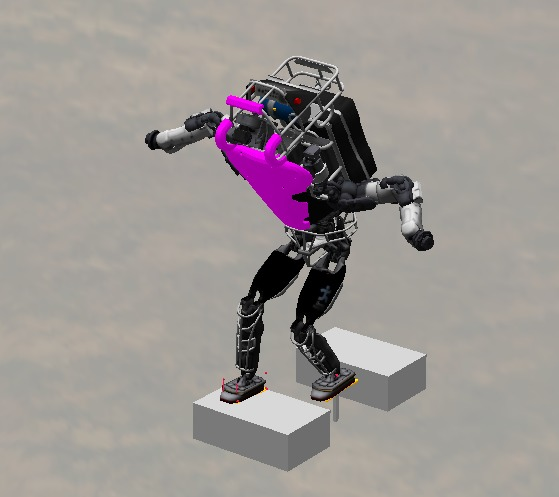
\includegraphics[height=0.8\textwidth]{atlas.jpg}
                \caption{Walking Robot \cite{wiedebach_walking_2016}}
                \label{fig:walking-robot}
            \end{figure}
        \end{column}
        \begin{column}{0.5\textwidth}
            \begin{figure}
                \centering
                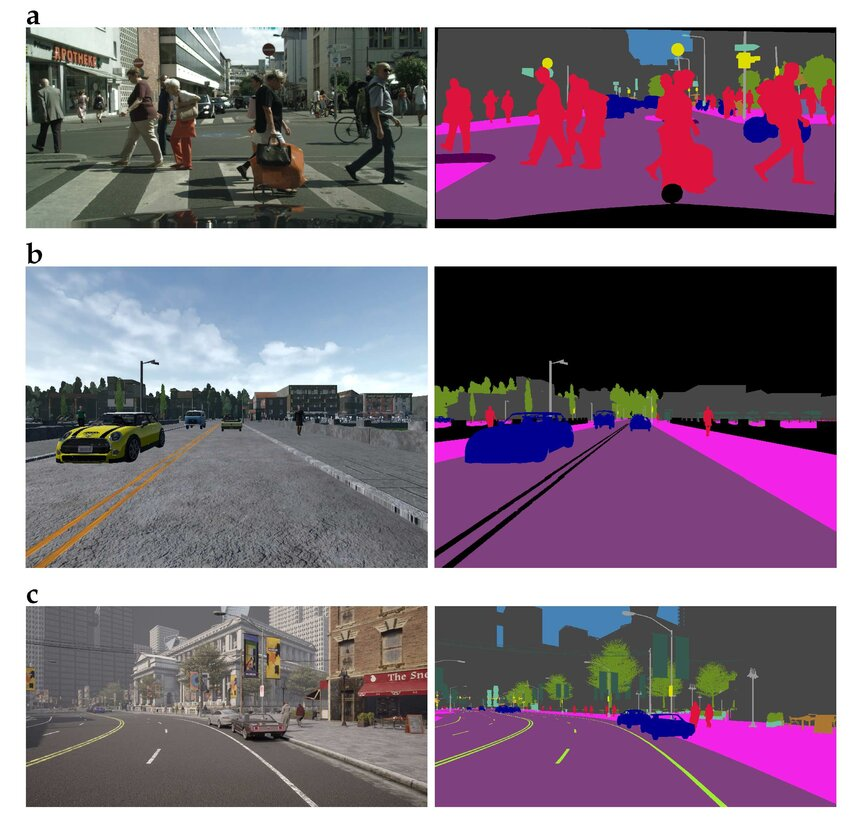
\includegraphics[height=0.8\textwidth]{tesla.jpg}
                \caption{Autonomous driving \cite{saha_practical_2023}}
                \label{fig:autonomous-driving}
            \end{figure}
        \end{column}
    \end{columns}
\end{frame}

\begin{frame}{Agent-Environment Interface}
    \begin{minipage}[c][2cm][c]{\textwidth}
        \only<1>{\begin{description}[labelsep=2cm]
            \item[Agent:] Decision-maker taking actions
            \item[Environment:] World which the agent interacts with
        \end{description}}
        \only<2>{\begin{description}
            \item[Action:] Move the agent can make in the environment
            \item[Observation:] Agent's perception of the environment
        \end{description}}
        \only<3>{\begin{description}
            \item[State:] Current situation or configuration of the environment
            \item[Reward:] Scalar value given to an agent as feedback for its actions
        \end{description}}
    \end{minipage}
    
    \tikzset{
    block/.style={rectangle, draw, text width=6em, text centered, minimum height=3em},
    action/.style={rectangle, color=white, fill=structure, text width=7em, text centered, minimum height=2em, rounded corners=5pt}}
    
    \begin{figure}
        \begin{tikzpicture}[very thick]
            % Nodes
            \node[block] (agent) {Agent};
            \node[block, right=5cm of agent] (environment) {Environment};
            \uncover<2->{\node[action, above=1cm of {$(agent)!0.5!(environment)$}] (actions) {Action};}
            \uncover<2->{\node[action, below=1cm of {$(agent)!0.5!(environment)$}] (observations) {Observation};}
            \uncover<3->{\node[below=0mm of actions] (action) {\small action $a_t$};}
            \uncover<3->{\node[above=0mm of observations] (new_state) {\small state $s_{t+1}$};}
            \uncover<3->{\node[below=0mm of observations] (reward) {\small reward $r_{t+1}$};}
            % Arrows
            \uncover<2->{\draw[-, color=structure] (agent.north) |- (actions.west);}
            \uncover<2->{\draw[->, color=structure] (actions.east) -| (environment);}
            \uncover<2->{\draw[-, color=structure] (environment.south) |- (observations.east);}
            \uncover<2->{\draw[->, color=structure] (observations.west) -| (agent.south);}
        \end{tikzpicture}
        \caption{The agent-environment interface \cite{sutton_reinforcement_2020}}
        \label{fig:agent-environment}
    \end{figure}
\end{frame}

\begin{frame}{Maze Example}
    \begin{columns}
        \begin{column}{0.5\textwidth}
            \begin{figure}
            \begin{tikzpicture}
                \filldraw[structure] (0.5,3.5) circle (0.2cm);
                \draw (3.5,4.5) node{-10};
                \fill[black] (2,2) rectangle (5,3);
                \fill[black] (2,1) rectangle (3,2);
                \draw (4.5,0.5) node{+10};
                \draw[step=1cm] (0,0) grid (5,5);
            \end{tikzpicture}
            \caption{Maze Example}
            \label{fig:maze-example}
            \end{figure}
        \end{column}
        \begin{column}{0.5\textwidth}
            \textbf{Agent:} 
            \begin{tikzpicture}[baseline=-0.5ex]
                \filldraw[structure] circle (0.2cm);
            \end{tikzpicture}
            
            \textbf{Actions:} $\{\boldsymbol{\uparrow}, \boldsymbol{\rightarrow}, \boldsymbol{\downarrow}, \boldsymbol{\leftarrow}\}$
            
            \textbf{States:} $\{(x, y) \mid x,y \in \{0, \dots, 4\}$
        \end{column}
    \end{columns}
\end{frame}

\begin{frame}{Returns and Value Functions}
    \begin{itemize}
        \item The agent’s job is to maximize cumulative reward, called the \alert{return}
        \begin{equation*}
            G_t = R_{t+1} + R_{t+2} + R_{t+3} + \dots
        \end{equation*}
        \begin{columns}
            \begin{column}{0.45\textwidth}
                \centering
                \textbf{state-value function}
                \begin{equation*}
                    v(s) = \mathbb{E} [G_t \mid S_t = s]
                \end{equation*}
                How good it is for the agent to be in a given state
            \end{column}
            \begin{column}{0.45\textwidth}
                \centering
                \textbf{action-value function}
                \begin{equation*}
                    q(s,a) = \mathbb{E} [G_t \mid S_t = s, A_t = a]
                \end{equation*}
                How good it is to perform a certain action in a given state
            \end{column}
        \end{columns}
        \vspace{5mm}
        \item A \alert{policy} is a strategy that the agent follows to decide actions based on the current state $\pi(s) \rightarrow a$
        \item Goal: select actions to maximize value $\rightarrow$ \alert{find optimal policy}
        \begin{equation*}
            \pi^*(s) = \underset{a}{\text{argmax }} q(s,a)
        \end{equation*}
    \end{itemize}
\end{frame}

%---------------------------------------------------------

\subsection{Q-Learning}
\begin{frame}{Q-Learning}
    \begin{itemize}
        \item \alert{Q-Learning} uses a Q-table with $S \times A$ entries to store the expected rewards for state-action pairs
        \begin{equation*}
            Q(S_t, A_t) \leftarrow Q(S_t, A_t) + \alpha \underbrace{\Bigl[R_{t+1} + \gamma \max_a Q(S_{t+1}, a) - Q(S_t, A_t)\Bigr]}_\text{Bellman error}
        \end{equation*}
        \item The \alert{Bellman error} is the difference between the current estimate of the Q-value for a state-action pair and the "true" Q-value
        \item The discount factor $\boldsymbol{\gamma}$ determines the importance of future rewards relative to immediate rewards
        \item The learning rate $\boldsymbol{\alpha}$ determines how quickly the agent learns from its experiences
    \end{itemize}
\end{frame}

%---------------------------------------------------------

\subsection{Limitations of standard RL}
\begin{frame}{Limitations of standard RL}
    \begin{itemize}
        \item Curse of dimensionality
        \begin{description}
            \item[Problem:] Tabular methods are impractical
        \end{description}
        \item Generalization across states
        \begin{description}
            \item[Problem:] Fail to generalize across similar states
        \end{description}
        \item Continuous state and action spaces
        \begin{description}
            \item[Problem:] Designed for continous domains
        \end{description}
    \end{itemize}
    \begin{block}{Solution}<2->
        Use a function approximator to estimate $Q(S,A)$
        \begin{itemize}
            \item[$\boldsymbol{\rightarrow}$] Deep Neural Network
        \end{itemize}
    \end{block}
\end{frame}

\section{Deep Q Networks}
\subsection{Workings of DQNs}
\subsection{Applications}

%---------------------------------------------------------
\begin{frame}[allowframebreaks]{References}
\bibliographystyle{ieeetr}
\bibliography{cognitive-algoritms-seminar}
\end{frame}

\end{document}